\documentclass[mathserif,blue]{beamer}
\usepackage{amssymb,tikz,amsmath}
\usetikzlibrary{arrows,calc,intersections,through,backgrounds,math,angles,shapes}
\usepackage[noindent,space]{ctex}%宏包加载
\usetheme{Boadilla}\beamersetaveragebackground{black!10}%主题设置
\setbeamersize{text margin left=1.3cm}\setbeamersize{text margin right=1.2cm}%页面尺寸
\newcommand\colorwordsa[1]{\textcolor[rgb]{0,.63,.91}{\small\heiti#1}}%彩色文字
\newcommand\colorwordsb[1]{\textcolor[rgb]{.75,.53,.21}{\small\heiti#1}}%彩色文字
\newcommand\threesides{\begin{picture}(14,12)\put(0,0){\qbezier(0,0)(0,8)(7,12)\qbezier(7,12)(14,8)(14,0)\qbezier(14,0)(7,-4)(0,0)}\end{picture}}%logo
\newlength\lengtha\newcommand\an[1][a]{\ensuremath{\{#1_n\}}}\newcommand\lines[1][1.2]{\,\underline{\mbox{\hspace{#1cm}}}\,}% 代码
\setbeamercolor{mycolor}{fg=black,bg=pink}\setbeamercolor{myupcol}{fg=white,bg=purple}\setbeamercolor{mylowcol}{fg=black,bg=pink}% 彩色盒子
\newcommand\beamercolortextbox[1]{\settowidth\lengtha{#1}\hspace{.5em}\raisebox{-.6ex}{\begin{beamercolorbox}[rounded=true,shadow=true,wd=\lengtha,colsep*=-.4ex]{mycolor}#1\end{beamercolorbox}}}
\newcommand\beamercolorlinebox[1]{\settowidth\lengtha{#1}\centerline{\begin{beamercolorbox}[rounded=true,shadow=true,wd=\lengtha]{mycolor}#1\end{beamercolorbox}}}
\begin{document}

\title{平面向量的实际背景及其基本概念}
\author{王崇宁}
\institute[四中]{郑州四中}
\logo{\threesides}
\maketitle


\begin{frame}{力}
\begin{columns}\begin{column}<1->{0.45\textwidth}
  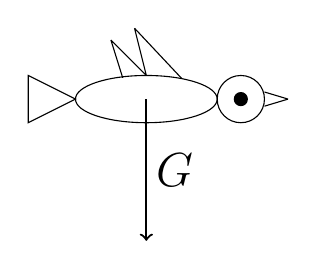
\begin{tikzpicture}[scale=.3]
    \draw(0,1)--(0,-1)--(2,0)--cycle;
    \draw(5,0)ellipse(3 and 1);
    \draw(9,0)circle(1);
    \draw(10,.3)--(11,0) (10,-.3)--(11,0);
    \fill[black](9,0) circle(.3);
    \draw (3.5,2.5)--(4,.9) (3.5,2.5)--(5,1) (4.5,3)--(5,1) (4.5,3)--(6.5,.87);\pause
    \draw[->,thick](5,0)--(5,-6);
    \node[right]at(5,-3){\LARGE$G$};
  \end{tikzpicture}
\end{column}\begin{column}<3->{0.45\textwidth}
  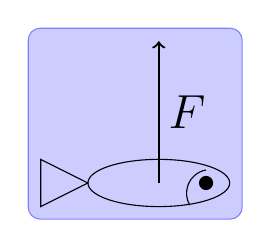
\begin{tikzpicture}[scale=.3,background rectangle/.style=
{draw=blue!50,fill=blue!20,rounded corners=1ex},show background rectangle]
    \draw(0,1)--(0,-1)--(2,0)--cycle;
    \draw(5,0)ellipse(3 and 1);
    \draw(7,.55)arc(100:210:1);
    \fill[black](7,0) circle(.3);\pause
    \draw[->,thick](5,0)--(5,6);
    \node[right]at(5,3){\LARGE$F$};
  \end{tikzpicture}
\end{column}\end{columns}
\end{frame}

\begin{frame}{力}
\begin{columns}\begin{column}<1->{0.55\textwidth}
  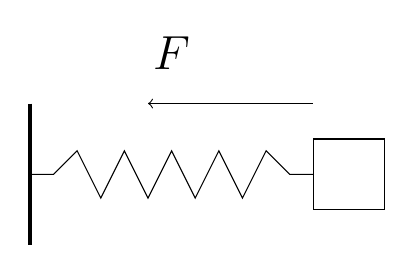
\begin{tikzpicture}[scale=.3]
    \draw[ultra thick](0,3)--(0,-3);
    \draw(0,0)--(1,0)--(2,1)--(3,-1)--(4,1)--(5,-1)--(6,1)--(7,-1)--(8,1)--(9,-1)--(10,1)--(11,0)--(12,0);
    \draw (12,-1.5)rectangle(15,1.5);
    \draw [<-](5,3)--(12,3);
    \node[above,thick]at(6,4){\LARGE$F$};
  \end{tikzpicture}
\end{column}\begin{column}<2->{0.4\textwidth}
  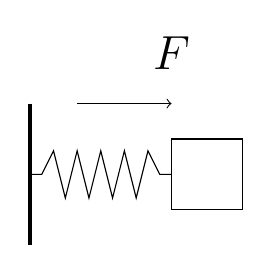
\begin{tikzpicture}[scale=.3]
    \draw[ultra thick](0,3)--(0,-3);
    \draw(0,0)--(.5,0)--(1,1)--(1.5,-1)--(2,1)--(2.5,-1)--(3,1)--(3.5,-1)--(4,1)--(4.5,-1)--(5,1)--(5.5,0)--(6,0);
    \draw (6,-1.5)rectangle(9,1.5);
    \draw [->](2,3)--(6,3);
    \node[above,thick]at(6,4){\LARGE$F$};
  \end{tikzpicture}
\end{column}\end{columns}
\end{frame}

\begin{frame}{从物理到数学}
在数学中,我们把这种\underline{既有大小},\underline{又有方向}的量叫做\colorwordsa{向量}。而把那些只有大小,没有方向的量(如年龄、身高、长度、面积、体积、质量等),称为\colorwordsa{数量}。
\end{frame}

\begin{frame}{几何表示:有向线段}
\begin{columns}\begin{column}<1->{0.65\textwidth}
  \colorwordsa{有向线段}$\overrightarrow{AB}$是以$A$为起点,以$B$为终点的线段。已知$\overrightarrow{AB}$,线段$AB$的长度也叫做有向线段$\overrightarrow{AB}$的长度,记作$|\overrightarrow{AB}|$. \par
的向线段包含三个要素:\colorwordsb{起点、方向、长度}.
\end{column}\begin{column}<2->{0.3\textwidth}
  \begin{tikzpicture}[scale=.5]
    \draw[thick,->](0,0)node[right]{$A$(起点)}--(4,3)node[right]{$B$(终点)};
    \fill[black,opacity=.8](0,0)circle(3pt);
  \end{tikzpicture}
\end{column}\end{columns}
\end{frame}

\begin{frame}{向量的表示}
  向量可以用有向线段表示。(这句话暗示我们向量并不等同于有向线段)向量$\overrightarrow{AB}$的大小称为\colorwordsa{模}(或者\colorwordsa{长度})。模为$0$的向量叫\colorwords{零向量},记作$\mathbf{0}$. 模为$1$的向量叫\colorwords{单位向量}。\par
  用有向线段的起点和终点字母表示向量,就记作$\overrightarrow{AB},\overrightarrow{CD}$. 向量也可以用小写字母表示,如$\bfmath{a},\bfmath{b},\bfmath{c},\cdots$
\end{frame}




\end{document}
黑体和手写体的$a$与$0$放在一页里以示强调 
在讲平行向量的时候说明向量与有向线段的区别,练习 在正六边行中向量平等于自身
在讲相等向量时讲述向量的平移不变性
\begin{columns}\begin{column}<1->{0.55\textwidth}
  
\end{column}\begin{column}<2->{0.4\textwidth}
  
\end{column}\end{columns}    \documentclass[12pt]{article}
\usepackage{ctex,amsmath}
\begin{document}

\end{document}
